\chapter{Results}

\label{Results}

This chapter presents the main outcomes of the proposed \ac{mcts}-based system for \ac{cb-ctt}, including its performance, feasibility, and evaluations of enhancements such as the diving strategy.

\section{Python vs PyPy Performance}

During the development and testing of the system, both standard Python and PyPy\footnote{A Just-In-Time (JIT) compiling alternative. Link: \url{https://pypy.org/}} were evaluated for performance. While both interpreters correctly executed the \ac{mcts} algorithm, the performance difference was substantial. PyPy called over 3 times more functions compared to Python.

Given the compute-intensive nature of \ac{mcts}, PyPy was ultimately chosen for running all the experiments and benchmarks.

\section{Feasibility}

The proposed system consistently produced feasible solutions across all tested configurations and datasets.

\section{\(C\) Parameter Behaviour}

The exploration constant \(C\) in the \ac{uct} formula (Formula \ref{uct_formula}) was varied across several orders of magnitude (from 0.1 to 1000), including the modified variant incorporating accumulated rewards (Formula \ref{modified_uct}). Surprisingly, the results showed that varying \(C\) had minimal impact on solution quality, which indicates a lower-than-expected sensitivity to node selection.

\section{Pruning}

The application of pruning during \ac{mcts} plays a crucial role in the effectiveness and efficiency of the search process.

Without pruning (Figure \ref{fig:without_pruning}), the search frequently explores solution paths that violate hard constraints. This is evident from the large number of iterations with hard constraint violations. The corresponding plot appears noisy and erratic, indicating that the algorithm repeatedly invests effort in exploring infeasible branches of the tree. Although some feasible solutions are eventually discovered, the overall search efficiency is compromised due to the continuous evaluation of invalid solutions.

Conversely, when pruning is applied (Figure \ref{fig:pruning}), the search is restricted to branches that satisfy all hard constraints. As a result, the hard constraint value remains consistently at zero throughout the iterations, reflecting that pruning effectively excludes infeasible regions from the search space. This restriction allows \ac{mcts} to focus on high-quality and valid solutions. The cleaner progression and stable constraint satisfaction not only accelerate convergence but also improve the overall robustness of the approach. 

While not depicted in this specific example, it is worth noting that simulations may still experience occasional hard constraint violations because pruning is applied to branches within the tree rather than across the entire search space.

\begin{figure}
 \centering
     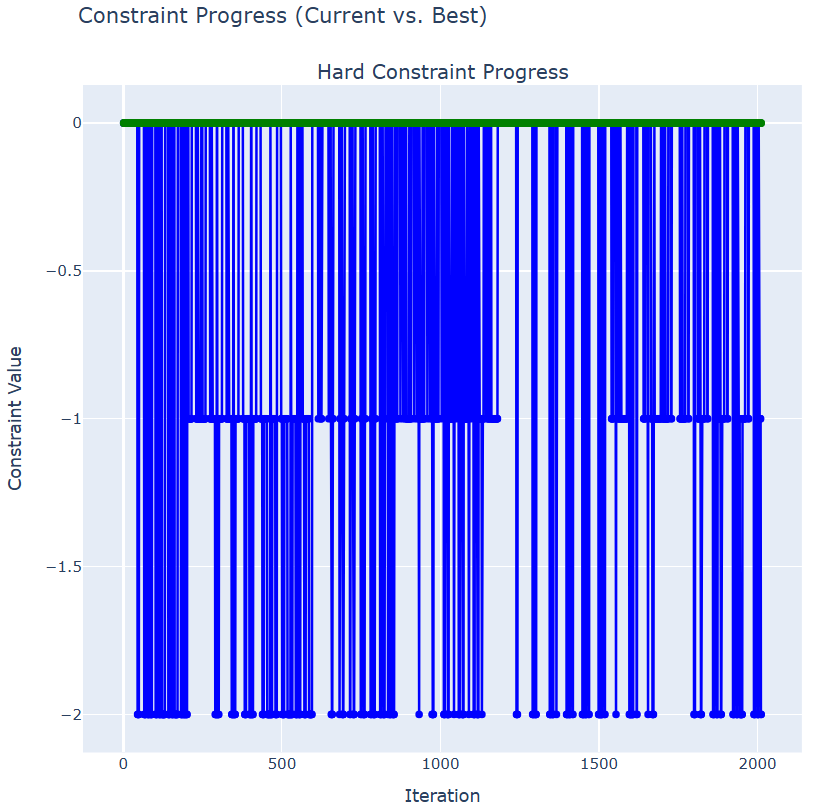
\includegraphics[width=0.7\columnwidth]{Results/without_pruning.png}
     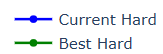
\includegraphics[width=0.2\columnwidth]{Results/pruning_caption.png}
     \caption{Hard constraint progress without pruning during 10 minutes.}
     \label{fig:without_pruning}
\end{figure}

\begin{figure}
 \centering
    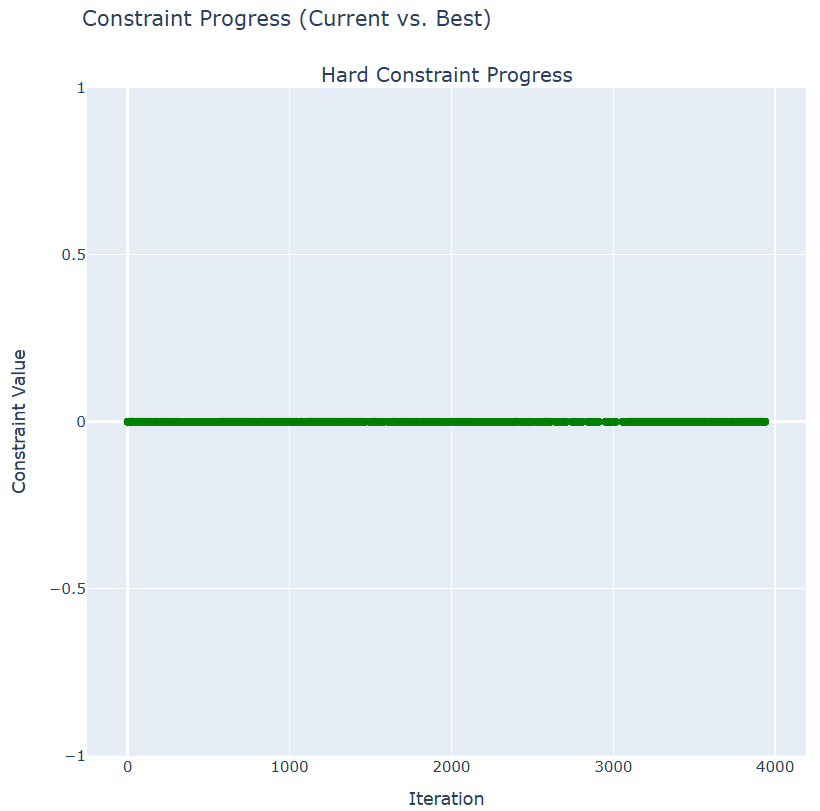
\includegraphics[width=0.7\columnwidth]{Results/pruning.png}
    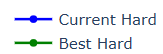
\includegraphics[width=0.2\columnwidth]{Results/pruning_caption.png}
    \caption{Hard constraint progress with pruning during 10 minutes.}
    \label{fig:pruning}
\end{figure}



\section{Diving strategy}

\section{Competition Results Comparison}

\begin{table}[h!]
\centering
\footnotesize
\begin{tabular}{ccccccccccccccccc}
\hline
& \multicolumn{3}{c}{\textbf{comp01}} & \multicolumn{3}{c}{\textbf{comp02}} & \multicolumn{3}{c}{\textbf{comp03}} & \multicolumn{3}{c}{\textbf{comp04}} & \multicolumn{3}{c}{\textbf{comp05}} \\
& avg & max & min & avg & max & min & avg & max & min & avg & max & min & avg & max & min \\
\textbf{Muller} & \textbf{5} & 5 & \textbf{5} & 61,3 & 70 & 51 & 94,8 & 103 & 84 & 42,8 & 48 & 37 & 343,5 & 379 & 330 \\
\textbf{Our Results} & & & & & & & & & & & & & & & \\
\end{tabular}

\centering
\footnotesize
\begin{tabular}{ccccccccccccccccc}
\hline
& \multicolumn{3}{c}{\textbf{comp06}} & \multicolumn{3}{c}{\textbf{comp07}} & \multicolumn{3}{c}{\textbf{comp08}} & \multicolumn{3}{c}{\textbf{comp09}} & \multicolumn{3}{c}{\textbf{comp10}} \\
& avg & max & min & avg & max & min & avg & max & min & avg & max & min & avg & max & min \\
\textbf{Muller} & \textbf{56,8} & 65 & \textbf{48} & \textbf{33,9} & 45 & \textbf{20} & 46,5 & 55 & 41 & \textbf{113,1} & 117 & 109 & \textbf{21,3} & 27 & \textbf{16} \\
\textbf{Our Results} & & & & & & & & & & & & & & & \\
\end{tabular}

\centering
\footnotesize
\begin{tabular}{ccccccccccccccccc}
\hline
& \multicolumn{3}{c}{\textbf{comp11}} & \multicolumn{3}{c}{\textbf{comp12}} & \multicolumn{3}{c}{\textbf{comp13}} & \multicolumn{3}{c}{\textbf{comp14}} & \multicolumn{3}{c}{\textbf{comp15}} \\
& avg & max & min & avg & max & min & avg & max & min & avg & max & min & avg & max & min \\
\textbf{Muller} & \textbf{0} & 0 & \textbf{0} & \textbf{351,6} & 367 & \textbf{333} & \textbf{73,9} & 81 & \textbf{66} & \textbf{61,8} & 69 & 59 & 94,8 & 103 & 84 \\
\textbf{Our Results} & & & & & & & & & & & & & & & \\
\end{tabular}

\centering
\footnotesize
\begin{tabular}{ccccccccccccccccc}
\hline
& \multicolumn{3}{c}{\textbf{comp16}} & \multicolumn{3}{c}{\textbf{comp17}} & \multicolumn{3}{c}{\textbf{comp18}} & \multicolumn{3}{c}{\textbf{comp19}} & \multicolumn{3}{c}{\textbf{comp20}} \\
& avg & max & min & avg & max & min & avg & max & min & avg & max & min & avg & max & min \\
\textbf{Muller} & \textbf{41,2} & 49 & \textbf{34} & \textbf{86,6} & 92 & \textbf{83} & 91,7 & 102 & 83 & \textbf{68,8} & 74 & \textbf{62} & \textbf{34,3} & 44 & \textbf{27}  \\
\textbf{Our Results} & & & & & & & & & & & & & & & \\
\end{tabular}

\centering
\footnotesize
\begin{tabular}{ccccccccccccccccc}
\hline
& \multicolumn{3}{c}{\textbf{comp21}} & \multicolumn{3}{c}{} &  \multicolumn{3}{c}{} & \multicolumn{3}{c}{} & \multicolumn{3}{c}{} \\
& avg & max & min &  &  &  &  &  &  &  &  &  &  &  &  \\
\textbf{Muller} & \textbf{108} & 121 & \textbf{103}  \\
\textbf{Our Results} & & &  \\
\hline
\end{tabular}
\caption{Comparison for comp01 to comp21}
\end{table}
